%!TEX root = ../thesis.tex
%*******************************************************************************
%****************************** Second Chapter *********************************
%*******************************************************************************

\chapter{Marco teórico}\label{chapter2}

\graphicspath{{Chapter2/Figs/}}


% {\color{magenta}Aquí debo ahondar más en lo que se plasma en este capítulo. Decir que en RL empezamos desde el planteamiento de MDP, y como se soluciona con RL, monte carlo
% te lleva a TD y eso s Q learning. luego de la versión para ambientes continuos y del estado del arte que es DQN. Por el lado de causalitdad }

En este capítulo se describen algunos conceptos fundamentales para entender
el problema atacado, la propuesta de solución y los métodos que 
se evalúan en los experimentos.
Dado que los dos campos que conducen este trabajo son
el aprendizaje por refuerzo y la causalidad, estos son
presentados de manera general en las siguientes dos
secciones.
La Sección \ref{rl-section} describe lo que es el aprendizaje
por refuerzo, el planteamiento del problema
como un proceso de decisión de Markov, las ecuaciones
fundamentales para su solución y algunos métodos para
resolverlo.
La Sección \ref{causation-section} contiene las ideas que se utilizan
con respecto al enfoque intervencionista de causalidad que se sigue en este trabajo, la definición de causalidad propuesta
por \cite{spirtes2000causation}, la 
representación de conocimiento en modelos gráficos 
causales y la definición de intervenciones en un modelo usando el operador $do(\cdot)$ \cite{pearl_2009}.

\section{Aprendizaje por refuerzo}\label{rl-section}

El aprendizaje por interacción es una idea esencial que subyace en casi todas la teorías
de aprendizaje e inteligencia \cite{sutton_barto_2018}.
Una perspectiva dentro del \textit{aprendizaje computacional} \cite{Goodfellow-et-al-2016} enfocada al aprendizaje dirigido a metas a través de interacciones es el \textit{aprendizaje por refuerzo}.

El aprendizaje por refuerzo se encarga de aprender el comportamiento de un agente 
de tal forma que se maximice una señal de recompensa numérica, esto es, a que un
agente aprenda a relacionar estados de su mundo a acciones. Al aprendiz o agente no se le 
dice qué acciones tomar, en cambio éste debe descubrir cuáles, al intentarlas, producen
una mayor recompensa. 
En la Figura \ref{fig:rl-outline} se muestra el esquema general de la interacción de un agente de RL con su mundo.

Las dos características más importantes que diferencían al
aprendizaje por refuerzo de otros paradigmas en el aprendizaje computacional son 
la búsqueda por prueba-y-error y la recompensa diferida. Que la recompensa sea diferida significa que el agente debe ser 
capaz de aprender cuales son acciones deseables basándose en una recompensa que puede ocurrir muy en el futuro.

\begin{figure}[h]
    \centering
    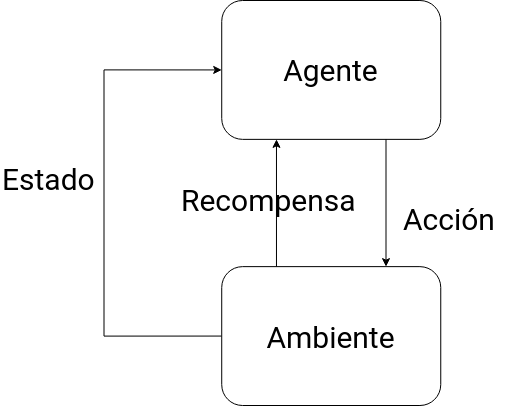
\includegraphics[scale=0.4]{Chapter2/Figs/agend_interaction.png}
   
    \caption{La idea general del RL es que un agente interactúa con un ambiente para
    aprender a partir de experiencias. Cada paso en el tiempo, el agente se encuentra
    en cierto estado $s\in \mathcal{S}$ y toma la acción $a \in \mathcal{A}$. Como
    resultado, el estado del mundo cambia y recibe una recompensa $r$.  \label{fig:rl-outline}}
\end{figure}

En las siguientes secciones primero se formaliza el problema de aprendizaje por refuerzo como
un problema de control óptimo para procesos de decisión de Markov incompletos (MDP por sus siglas en inglés) y luego se
describe el algoritmo \textit{Q-learning}, cuyo desarrollo involucró un gran avance en esta área de la IA  .

\subsection{Procesos de decisión de Markov}


Los procesos de decisión de Markov (MDP) son un marco de trabajo para
definir el problema de aprender
mediante interacciones como 
alcanzar una meta. El tomador de 
decisiones es llamado \textit{agente}.
El agente interactúa con un mundo, que
abarca todo fuera de éste, y se
conoce como \textit{ambiente}.
Estos dos elementos
interactúan continuamente, el agente
selecciona \textit{acciones} y
el ambiente responde a estas 
acciones presentando nuevos 
\textit{estados} al agente. Además,
existen \textit{recompensas},
las cuales son valores numéricos 
que el agente busca maximizar con
el paso del tiempo mediante la 
selección de sus acciones.

Formalmente, un MDP es una tupla $< \mathcal{S}, \mathcal{A}, \mathcal{P}, \mathcal{R}, \gamma>$ tal que

\begin{itemize}
    \item $\mathcal{S}$ es el conjunto de estados, donde $s_t$ denota el estado $s\in \mathcal{S}$ en el tiempo $t$.
    \item $\mathcal{A}$ es el conjunto de acciones, donde $a_t \in \mathcal{A}$
    denota la acción realizada en un estado $s$ en el tiempo $t$.
    \item $\mathcal{P}_{ss'}^{a}: \mathcal{S}\times \mathcal{A} \times \mathcal{S} \rightarrow [0, 1]$ (también denotada por $\mathcal{P}$) es una función de probabilidad de transición de pasar del estado $s \in \mathcal{S}$ al estado $s' \in \mathcal{S}$ cuando se toma la acción $a$.% en el tiempo $t$.
    \item $\mathcal{R}_{ss'}^{a}: \mathcal{S} \times \mathcal{A} \times \mathcal{S} \rightarrow \mathbb{R}$ (también denotada por $\mathcal{R}$) es la función de recompensa inmediata que el agente recibe después de pasar de $s$ a $s'$, habiendo tomado la acción $a$.
    \item $\gamma \in [0,1]$ es el factor de descuento que sirve para
    calcular el retorno esperado con descuento.
\end{itemize}


Además de estos componentes, un sistema de aprendizaje por refuerzo subsume otros elementos como: una \textit{política} y una \textit{función de valor}. Por lo tanto, la tupla se puede reescribir como $< \mathcal{S}, \mathcal{A}, \mathcal{P}, \mathcal{R}, \gamma, \pi, f>$, donde los últimos elementos representan la política y la función de valor, respectivamente. Una política es una función $\pi$ que mapea estados
a acciones y que maximiza alguna medida de refuerzo a largo plazo. Mientras que la recompensa expresa lo que es bueno
de manera inmediata, una función de valor especifica lo que
es bueno a la larga. 
%Un modelo consiste del conocimiento de la
%función de probabilidad de transición $\mathcal{P}$ y
%de la función de recompensa $\mathcal{R}$.
El aprendizaje por refuerzo aprende las funciones de valor o la política mientras 
interactúa con el ambiente.
% %  
% % Whereas the reward signal indicates what is good in an immediate sense, a value
% % function specifies what is good in the long run. Roughly speaking, the value of a state is the total amount of reward an agent can expect to accumulate over the future, starting from that state.

% % Es la recompensa total que un agente puedeesperar acumular empezando en un estados(V(s)) oen un estado haciendo una acona(Q(s,a))

% % 

% % element of some reinforcement learning systems is a model of
% % the environment. This is something that mimics the behavior of the environment, or more generally, that allows inferences to be made about how the environment will behave.
 Un paso en la interacción de un agente con el ambiente se puede ver como que dado un estado $s_t \in \mathcal{S}$ y una
acción $a_t\in \mathcal{A}$, el agente pasa a un nuevo
estado $s_{t+1} \in \mathcal{S}$ y recibe una recompensa
$r_{t+1}$.
% Una política $\pi$ es una función de los estados percibidos del ambiente a acciones que se toman cuando se está en esos estados ($\pi : \mathcal{S} \rightarrow \mathcal{A}$).
% El problema fundamental en los MDP es
% encontrar una política óptima; esto es, 
% aquella que maximiza la recompensa esperada por el agente a largo plazo.
En RL, la meta del agente está formalizada
en términos de la señal de recompensa que
envía el ambiente al agente. En cada paso $t$, sin pérdida de generalidad, la recompensa es un número real $r_t \in \mathbb{R}$. Aunque las funciones de valor pueden estar en el dominio de $\mathbb{C}$ como en \cite{complexRLhamagami}. La meta de un agente
es maximizar la recompensa total recibida.
Esto significa, que no solo se maximiza la recompensa inmediata sino la recompensa acumulada a largo plazo.

En general, se busca maximizar el \textit{retorno
esperado}, donde el retorno, denotado por $R_t$, se define como alguna función de la secuencia de recompensas. 
El \textit{retorno esperado con descuento} es la suma acumulada de recompensas descontadas. El factor de descuento $\gamma$
define que tantas recompensas en el 
futuro son consideradas. Si $\gamma = 0$
solo la recompensa inmediata es
tomada en cuenta.

\begin{equation}
\label{eq:retorno-esperado}
R_t = r_{t+1} + \gamma r_{t+2} + \gamma^2 r_{t+3} + \gamma^3 r_{t+4} + \dots = 
\sum_{k = 0}^\infty \gamma^{k} r_{t+k+1}
\end{equation}

Si se tiene un punto terminal se llaman tareas \textit{episódicas}, si no se tiene se conocen como tareas \textit{continuas}.

% \subsection{Política y funciones de valor}

Una política, denotada por $\pi(s, a)$, describe una manera de actuar. Es una función que mapea un estado $s$ y una acción $a$ a la probabilidad de tomar esa acción en ese estado.
Por lo tanto para un estado dado, 
$\sum_a \pi (s, a) = 1$. El problema fundamental en los MDP es encontrar una política óptima $\pi^*$, es decir, aquella que maximiza la recompensa que espera recibir el agente a largo plazo.
A veces es escrita como $\pi^*(s) = a$, la cual es una relación de estados a las acciones óptimas en esos estados.

Para aprender la política óptima, se utilizan las \textit{funciones de valor}. Existen dos tipos de funciones de valor: la \textit{función de valor de estado},
denotada por $V(s)$, y la \textit{función de valor de acción}, expresada como $Q(s, a)$.

La \textit{función de valor de estado} describe el valor de un estado al seguir una política. Es el retorno esperado partiendo del estado $s$, actuando de acuerdo
a la política $\pi$

\begin{equation}\label{eq:state-value-func}
V^\pi(s) = \mathbb{E}_\pi[R_t | s_t = s].    
\end{equation}


La función de valor no necesariamente es la misma para dos políticas diferentes
en un mismo ambiente.  El valor del estado
cambia dependiendo del comportamiento del agente, ya que la manera de actuar
en un estado en particular afecta cuánta recompensa se espera recibir.
La razón de usar el valor esperado  es porque existe aleatoriedad en lo que
sucede después de llegar a un estado. Se puede contar con una política estocástica, lo que significa que se necesitan combinar los resultados de 
todas las acciones que se toman. Además, la función de transición puede ser estocástica, lo cual implica cierta incertidumbre de llegar a cualquier 
estado.

La otra función de valor que se utiliza es la \textit{función de valor de acción}.
La función de valor de acción define el valor de 
tomar una acción en algún estado cuando se sigue cierta política. Es el
retorno esperado dados un estado y una acción bajo la política $\pi$

\begin{equation}\label{eq:action-value-func}
Q^\pi (s,a) = \mathbb{E}[R_t | s_t = s, a_t = a].    
\end{equation}

Las funciones de valor óptimas se definen en las ecuaciones \ref{eq:optimal-value-function}
y \ref{eq:optimal-action-function}.

\begin{equation}
\label{eq:optimal-value-function}
V^*(s) = \max_{\pi} V^\pi(s).
\end{equation}
\begin{equation}
\label{eq:optimal-action-function}
    Q^*(s, a) = \max_{\pi} Q^\pi (s,a).
\end{equation}


Las funciones anteriores pueden ser expresadas mediante las \textit{ecuaciones de optimalidad de Bellman} \cite{bellman1966dynamic}.
Las ecuaciones de Bellman están presentes en casi todos lo métodos de RL y es importante conocer de donde surgen para comprender estos algoritmos. Por lo tanto, a continuación se muestra la obtención de las ecuaciones
de Bellman como lo muestra \cite{greaves}.

Las funciones $\mathcal{P}_{ss'}^a$ y $\mathcal{R}_{ss'}^a$ son la probabilidad de transición y la recompensa esperada, respectivamente. La primera se define como
$\mathcal{P}_{ss'}^a = P(s_{t+1} = s' | s_t = s, a_t = a)$,
y la segunda como
$\mathcal{R}_{ss'}^a = \mathbb{E}[r_{t+1} | s_t = s, s_{t+1} = s', a_t = a]$.

Usando la función de retorno esperado con descuento, se puede
reescribir la ecuación \ref{eq:state-value-func} como

\begin{equation}
V^\pi(s) = \mathbb{E}_\pi[r_{t+1} + \gamma r_{t+2} + \dots | s_t = s] = \mathbb{E}_{\pi}[\sum_{k = 0}^\infty \gamma^{k} r_{t+k+1} | s_t =s].
\end{equation}


Si se deja fuera de la suma la recompensa más antigua, se tiene
\begin{equation}
V^\pi(s) = \mathbb{E}_\pi[r_{t+1} + \gamma \sum_{k = 0}^\infty \gamma^{k} r_{t+k+2} | s_t =s].
\end{equation}

El valor esperado describe el retorno esperado que se obtiene si se parte del estado $s$ siguiendo la política $\pi$.
El valor esperado puede ser escrito explícitamente mediante la suma de todas
las acciones posible y todos los posible estados, por lo tanto se tienen las ecuaciones
\ref{eq:valor-esperado-recompensa-inmediata} y \ref{eq:valor-esperado-recompensas-siguientes}.

\begin{equation}
\label{eq:valor-esperado-recompensa-inmediata}
\mathrm{E}_\pi[r_{t+1}| s_t=s] = \sum_a \pi(s,a) \sum_{s'}\mathcal{P}_{ss'}^a\mathcal{R}_{ss'}^a,    
\end{equation}
\begin{equation}
\label{eq:valor-esperado-recompensas-siguientes}
\mathbb{E}_\pi[\gamma \sum_{k = 0}^\infty \gamma^{k} r_{t+k+2} | s_t =s] =
\sum_a \pi(s,a) \sum_{s'}\mathcal{P}_{ss'}^a \gamma \mathbb{E}_\pi[\sum_{k = 0}^\infty \gamma^{k} r_{t+k+2} | s_{t+1} = s']    
\end{equation}


Con las ecuaciones \ref{eq:valor-esperado-recompensa-inmediata} y \ref{eq:valor-esperado-recompensas-siguientes}, se puede reescribir $V^\pi(s)$ de la
siguiente forma
\begin{equation}
\label{eq:state-value-func-extended}
V^\pi(s) = \sum_a \pi(s,a) \sum_{s'}\mathcal{P}_{ss'}^a [\mathcal{R}_{ss'}^a +
\gamma \mathbb{E}_\pi[\sum_{k = 0}^\infty \gamma^{k} r_{t+k+2} | s_{t+1} = s']].
\end{equation}

La última parte de la ecuación \ref{eq:state-value-func-extended} tiene
la misma forma que la ecuación \ref{eq:state-value-func}. Por lo tanto, sustituyéndola, se tiene

\begin{equation}\label{eq:bellman-state-val}
    V^\pi(s) = \sum_a \pi(s,a) \sum_{s'}\mathcal{P}_{ss'}^a [\mathcal{R}_{ss'}^a + \gamma V^\pi(s')].
\end{equation}

La ecuación de Bellman para la función de valor de acción se deriva de la misma manera.

\begin{equation}\label{eq:bellman-acion-val}
    Q^\pi(s, a) = \sum_{s'}\mathcal{P}_{ss'}^a [\mathcal{R}_{ss'}^a + \gamma \pi(s',a')Q^\pi(s', a')].
\end{equation}

Las ecuaciones de Bellman permiten expresar valores de estados como
valores de otros estados, es decir, si se conoce el valor de $s_{t+1}$, se puede calcular $s_t$. A partir de las ecuaciones \ref{eq:bellman-state-val} y \ref{eq:bellman-acion-val} los valores óptimos de
las funciones de valor se describen en las ecuaciones \ref{eq:optimal-value-f} y \ref{eq:optimal-action-value-f}.

\begin{equation}
\label{eq:optimal-value-f}
V^*(s) = \max_{a}\sum_{s'}\mathcal{P}_{ss'}^a[\mathcal{R}_{ss'}^a + \gamma V^*(s')],
\end{equation}

\begin{equation}
\label{eq:optimal-action-value-f}
Q^*(s,a) = \sum_{s'}\mathcal{P}_{ss'}^a[\mathcal{R}_{ss'}^a + \gamma \max_{a'}Q^*(s',a')].
\end{equation}


Un MDP busca la solución a las ecuaciones de Bellman, lo que equivale a encontrar
la política óptima. Si $\mathcal{P}$ y $\mathcal{R}$ son conocidas, i.e., se cuenta con el \textit{modelo} de un MDP, se puede resolver mediante programación dinámica o programación lineal. En caso contrario, cuando el modelo no es conocido, se utiliza aprendizaje por refuerzo.
% Una política $\pi$ es una función de los estados percibidos del ambiente a acciones que se toman cuando se está en esos estados ($\pi : \mathcal{S} \rightarrow A$). 
% Whereas the reward signal indicates what is good in an immediate sense, a value
% function specifies what is good in the long run. Roughly speaking, the value of a state is the total amount of reward an agent can expect to accumulate over the future, starting from that state.

% \subsection{Método Monte Carlo}\label{subsection-montecarlo}

% El método Monte Carlo es un enfoque que busca resolver problemas
% de aprendizaje por refuerzo con tareas episódicas, donde 
% no existe un modelo del ambiente. 
% Es un método iterativo y converge a la política
% al incrementar el número de episodios.

% Existe una tabla $Q$ que almacena el valor de acción para cada posible
% par de estado-acción. El valor es el promedio sobre
% todos los retornos, que han sido obtenidos durante todos los episodios. 
% Un elemento de la tabla es actualizado cada vez que un par estado-acción
% es visitado por el agente. La ecuación de actualización se muestra en la 
% siguiente ecuación, donde $N(s_t, a_t)$ es el número de visitas al 
% par estado-acción $(s_t, a_t)$.

% \[
% Q(s_t, a_t) = Q(s_t, a_t) + \frac{1}{N(s_t, a_t)} (R_t - Q(s_t, a_t)).
% \]

% Los diferentes retornos pueden 
% ser ponderados por un peso $\alpha$.
% En vez de tomar el promedio
% verdadero, retornos recientes pueden tener un peso mayor o menor

% \begin{equation}\label{eq:montecarlo-update}
% \begin{split}
% Q(s_t, a_t) &= Q(s_t, a_t) + \alpha(R_t - Q(s_t, a_t))\\
% &= (1-\alpha)Q(s_t, a_t) + \alpha R_t.
% \end{split}
% \end{equation}

% El método Monte Carlo itera sobre episodios. Durante el paso de evaluación, el 
% agente actúa de acuerdo a la política $\pi$ de un episodio. Cuando el 
% episodio se termina, el agente recolecta una secuencia de experiencia $s_1, a_1, r_1, s_2, \dots, s_t$ y puede actualizar la tabla $Q$ de acuerdo
% con ésta.
% Para cada par estado-acción en la secuencia, se obtiene el retorno 
% esperado $R_t$ y se actualiza el elemento correspondiente en la tabla $Q$ 
% de acuerdo con la ecuación \ref{eq:montecarlo-update}.
% Durante el paso de mejora,  la
% política $\pi$ se actualiza de acuerdo a la tabla $Q$. En la siguiente iteración,
% el paso de evaluación se realiza con la política nueva que sea obtiene de la
% actualización.

% Normalmente, la política de actualización básica es una política voraz. El agente
% siempre elige la acción con el máximo valor de acción. Sin embargo, explotar la acciones vorazmente con el conocimiento actual puede conducir a que el
% agente quede atascado en una política no óptima. Para evitar 
% este caso, acciones exploratorias deben tomarse en cuenta de vez en cuando.
% Una política es llamada $\epsilon$-greedy, si la mejor acción actual se toma 
% con una probabilidad de $1-\epsilon$ y una acción aleatoria se toma con una 
% probabilidad $\epsilon$. La ecuación de la política $\epsilon$-greedy
% se puede definir de la siguiente manera

% \begin{equation}\label{eq:epsilongreedy}
% \pi(s,a) = 
%   \begin{cases} 
%       1 - \epsilon + \frac{\epsilon}{|\mathcal{A}|} & \mbox{si } a= 
%       \argmax_{a \in \mathcal{A}} 
%       Q(s,a)   \\
%       \frac{\epsilon}{|\mathcal{A}|} & \mbox{ en otro caso }
%   \end{cases}
% \end{equation}

% $\epsilon$ es un valor entre 0 y 1 y pondera la relación entre
% exploración y explotación.

\subsection{Métodos de diferencias temporales}

Una idea central e importante en RL es el aprendizaje 
a través de diferencias temporales (TD por sus siglas en inglés).
El aprendizaje TD es una combinación de ideas del método Monte Carlo y programación dinámica. 
% Los métodos de diferencias 
% temporales pueden aprender de experiencia sin 
% un modelo del ambiente como en los Monte Carlo. Por otro lado, 
% al igual que en programación dinámica,
% las actualizaciones de los métodos TD se basan en otros 
% estimados aprendidos, sin esperar a una salida final.
La ventaja de los métodos TD es que se pueden aplicar a tareas de aprendizaje por refuerzo en línea y continuas.
La política se actualiza cada paso de tiempo $t$ por lo que no se necesitan
 episodios completos (como en programación dinámica). Además, no se requiere el modelo del ambiente ni el sistema de recompensas (igual que en el método Monte Carlo).
%  Mientras que con programación dinámica se necesita conocer la función de transición y el sistema de recompensas el método Monte Carlo es un enfoque que busca resolver problemas
% de aprendizaje por refuerzo con tareas episódicas, donde 
% no existe un modelo del ambiente. 

% Es un método Monte Carlo es iterativo y converge a la política al incrementar el número de episodios.
% Existe una tabla $Q$ que almacena el valor de acción para cada posible
% par de estado-acción. El valor es el promedio sobre
% todos los retornos, que han sido obtenidos durante todos los episodios. 
% Un elemento de la tabla es actualizado cada vez que un par estado-acción
% es visitado por el agente.

En los métodos TD, al igual que en el Monte Carlo, el retorno esperado verdadero $R_t$ no está disponible
y es aproximado con un valor TD-target. El TD-target se determina con la suma de la recompensa inmediata y el valor esperando con descuento del 
siguiente estado $r_{t+1} + \gamma V(s_{t+1})$. El error que mide la diferencia entre el valor del estado $s_t$ ($V(s_t)$) y el estimado $r_{t+1} + \gamma V(s_{t+1})$ se llama TD-error. El Algoritmo \ref{alg:TD-algo} muestra un esquema general para los métodos que siguen la idea de actualizar la función de valor usando el TD-error.

\begin{mialgoritmo}[H]
  	\caption{Algoritmo general de los métodos TD}
	\label{alg:TD-algo}
  \begin{algorithmic}[1]
  \setstretch{1}
  \REQUIRE La política $\pi$ a ser evaluada, $\alpha \in (0,1]$.
  \STATE Inicializar arbitrariamente $V(s)$, para todo $s\in \mathcal{S}$ excepto donde $V(terminal) = 0$.
  
  \FOR{$episodio = 1, \dots, M$}
    \STATE Inicializar $s_0$.
    \FOR{$t = 0, \dots, T$}
    \STATE $a_{t} \leftarrow$ acción dada por $\pi$ para $s_t$.
    \STATE Tomar acción $a_t$ y observar $r_{t+1}, s_{t+1}$.
    \STATE $V(s_t) \leftarrow V(s_t) + \alpha\underbrace{[\underbrace{r_{t+1} + \gamma V(s_{t+1})}_{TD-target} - V(s_t)]}_{TD-error}$.
    \STATE $s_t \leftarrow s_{t+1}$.
    \ENDFOR
  \ENDFOR
  \end{algorithmic}
\end{mialgoritmo}



% \RestyleAlgo{boxruled}
% \begin{mialgoritmo}[!hbt]
% 	\caption{Algoritmo general de los métodos TD}
% 	\label{alg:TD-algo}
	
	
% 	\SetAlgoLined\DontPrintSemicolon
%     \SetAlgoHangIndent{0.5em}
% 	%\scriptsize
% 	\SetAlFnt{\large} 
%     \SetKwData{patterns}{\textit{PS}}
% 	\SetKwInOut{Input}{Entrada}
	
% 	\Input{La política $\pi$ a ser evaluada, $\alpha \in (0,1]$.}
% 	\BlankLine
	
%     Inicializar arbitrariamente $V(s)$, para todo $s\in \mathcal{S}$ excepto donde $V(terminal) = 0$\;
% 	Repetir por cada episodio:\;
% 	\hspace{0.5cm}Inicializar $s_t$\;
% 	\hspace{0.5cm}Repetir por cada paso del episodio:\;
% 	\hspace{1cm}$a_t \leftarrow$ acción dada por $\pi$ para $s_t$\;
% 	\hspace{1cm}Tomar acción $a_t$, observar $r_{t+1}$, $s_{t+1}$\;
% 	\hspace{1cm}$V(s_t) \leftarrow V(s_t) + \alpha\underbrace{[\underbrace{r_{t+1} + \gamma V(s_{t+1})}_{TD-target} - V(s_t)]}_{TD-error}$\;
%     \hspace{1cm}$s_t \leftarrow s_{t+1}$\;
%     \hspace{0.5cm}hasta que $s_t$ sea terminal o inválido\;
% \end{mialgoritmo}

% \subsection{Aprendizaje por refuerzo profundo}
% \subsubsection{Deep Q Network}

El algoritmo $Q$-learning \cite{watkins1992q} es un método de control TD \textit{fuera de política}, es decir,
la política $\pi$ no se utiliza, de manera explícita, para actualizar la tabla $Q$. 
La regla de actualización del $Q$-learning está dada por 

\begin{equation}\label{eq:q-learning-update}
Q(s_t, a_t) \leftarrow Q(s_t, a_t) + \alpha[r_{t+1} + \gamma \max_a Q(s_{t+1}, a) - Q(s_t, a_t)]
\end{equation}



Normalmente, la política para la selección de acciones es una política voraz. El agente
siempre elige la acción con el máximo valor de acción. Sin embargo, explotar la acciones vorazmente con el conocimiento actual puede conducir a que el
agente quede ``atascado'' en una política no óptima. Para evitar 
este comportamiento, se deben tomar en cuenta acciones exploratorias de vez en cuando.
Una política es llamada $\epsilon$-greedy, si la mejor acción actual se toma 
con una probabilidad de $1-\epsilon$ y una acción aleatoria se toma con una 
probabilidad $\epsilon$. La ecuación de la política $\epsilon$-greedy
se puede definir de la siguiente manera

\begin{equation}\label{eq:epsilongreedy}
\pi(s,a) = 
  \begin{cases} 
      1 - \epsilon + \frac{\epsilon}{|\mathcal{A}|} & \mbox{si } a= 
      \argmax_{a \in \mathcal{A}} 
      Q(s,a)   \\
      \frac{\epsilon}{|\mathcal{A}|} & \mbox{ en otro caso }
  \end{cases}
\end{equation}

$\epsilon$ es un valor entre 0 y 1 y pondera la relación entre
exploración y explotación.

En general, el algoritmo Q-learning consiste de de los siguientes pasos:
1) se inicializa la tabla $Q$ que relaciona los estados a valores de las acciones,
2) en un paso de tiempo $t$ del episodio el agente interactúa con su ambiente al realizar una acción $a_t$ de acuerdo con una política $\epsilon$-greedy (ecuación \ref{eq:epsilongreedy}) y obtiene una señal de recompensa $r_{t+1}$ y una observación $s_{t+1}$, y finalmente 3) actualiza los valores
correspondientes de la tabla $Q$ usando la ecuación \ref{eq:q-learning-update}. El método
se explica a detalle en el Algoritmo \ref{alg:q-algo}.

\begin{mialgoritmo}[H]
  	\caption{$Q$-learning}
	\label{alg:q-algo}
  \begin{algorithmic}[1]
  \setstretch{1}
  \REQUIRE $\alpha \in (0,1]$, $\epsilon \in (0, 1]$.
  \STATE Inicializar arbitrariamente $Q(s,a)$, para todo $s\in \mathcal{S}$ excepto donde $Q(terminal, \cdot) = 0$.
  
  \FOR{$episodio = 1, \dots, M$}
    \STATE Inicializar $s_0$.
    \FOR{$t = 0, \dots, T$}
    \STATE Elegir $a_t$ usando una política derivada de $Q$ (e.g., $\epsilon$-greedy).
    \STATE Tomar acción $a_t$ y observar $r_{t+1}, s_{t+1}$.
    \STATE $Q(s_t, a_t) \leftarrow Q(s_t, a_t) + \alpha [r_{t+1} + \gamma \max_a Q(s_{t+1}, a) - Q(s_t, a_t)]$.
    \STATE $s_t \leftarrow s_{t+1}$.
    \ENDFOR
  \ENDFOR
  \RETURN $Q$
  \end{algorithmic}
\end{mialgoritmo}

% \RestyleAlgo{boxruled}
% \begin{mialgoritmo}[!hbt]
% 	\caption{Algoritmo $Q$-learning}
% 	\label{alg:q-algo}
	
	
% 	\SetAlgoLined\DontPrintSemicolon
%     \SetAlgoHangIndent{0.5em}
% 	%\scriptsize
% 	\SetAlFnt{\large} 
%     \SetKwData{patterns}{\textit{PS}}
% 	\SetKwInOut{Input}{Entrada}
	
% 	\Input{$\alpha \in (0,1]$, $\epsilon \in (0, 1]$}
% 	\BlankLine
	
%     Inicializar arbitrariamente $Q(s,a)$, para todo $s\in \mathcal{S}$ excepto donde $Q(terminal, \cdot) = 0$\;
% 	Repetir por cada episodio:\;
% 	\hspace{0.5cm}Inicializar $s_t$\;
% 	\hspace{0.5cm}Repetir por cada paso del episodio:\;
% 	\hspace{1cm}Elegir $a_t$ usando una política derivada de $Q$ (e.g., $\epsilon$-greedy)\;
% 	\hspace{1cm}Tomar acción $a_t$, observar $r_{t+1}$, $s_{t+1}$\;
% 	\hspace{1cm}$Q(s_t, a_t) \leftarrow Q(s_t, a_t) + \alpha [r_{t+1} + \gamma \max_a Q(s_{t+1}, a) - Q(s_t, a_t)]$\;
%     \hspace{1cm}$s_t \leftarrow s_{t+1}$\;
%     \hspace{0.5cm}hasta que $s_t$ sea terminal o inválido\;
% \end{mialgoritmo}

\subsection{Q-learning profundo}

A pesar de que el algoritmo Q-learning resuelve muchos problemas, 
le es difícil hacer frente a situaciones donde el tamaño del conjunto de estados
es muy grande. Por ejemplo, en algunos videojuegos se puede tener una gran variedad
de imágenes diferentes, por lo que  si se decide a usar pixeles como 
estados individuales es fácil notar que se tiene que seguir la pista de muchos
estados y se tienen que aproximar muchos valores. 
Una solución a este problema es usar una función que se aproxime a aquella que relaciona
el par estado-acción a un valor.
Existen diversas formas de representar y entrenar dicha función, la que 
se explora en esta sección es usando una red neuronal profunda \cite{lapan_2020, Goodfellow-et-al-2016}.

Los autores en \cite{mnih2013playing} adaptaron el método Q-learning 
para que éste aproveche el uso de redes neuronales profundas como aproximadores
de funciones no lineales y un \textit{búfer de repetición} para estabilizar 
el aprendizaje. Este método es conocido como Q-learning profundo o red Q profunda (DQN por sus siglas en inglés).
La primera versión del algoritmo DQN fue aplicada al dominio de los videojuegos de Atari \cite{bellemare2013arcade}. De manera muy general, la red profunda recibe como entrada un conjunto de fotogramas a escala de grises de un videojuego, que son procesados por varias capas convolucionales para
extraer características del espacio y tiempo. El último mapa de características
de las capas convolucionales es procesado por varias capas completamente conectadas, que codifican los efectos de las acciones.

Son tres los elementos que forman las bases que permitieron mostrar
la eficiencia y efectividad de este enfoque en ambientes complejos: el uso de una política $\epsilon$-greedy, un búfer de repetición o experiencia de repetición \cite{lin1993reinforcement} y una red objetivo.
El búfer cíclico de experiencias de repetición guarda transiciones de la forma 
$(s_t, a_t, s_{t+1}, r_{t+1})$, permitiendo que un agente de RL 
tome muestras de éste y entrene sobre datos previamente observados. 
Esto no sólo reduce la cantidad de interacciones necesarias con el ambiente,
también permite obtener lotes de muestras, reduciendo la varianza de 
las actualizaciones de aprendizaje. 
% Además, al tomar muestras de una memoria
% muy grande, se rompen las correlaciones temporales que pueden afectar negativamente al algoritmo de RL.
El segundo método importante es el uso de una red objetivo que inicialmente contiene los pesos de la red que representa la política, sin embargo se mantiene
fija por un periodo largo de tiempo.
En vez de tener que calcular el error TD basándose en los estimados
oscilantes de los valores Q, la red de la política usa la red objetivo fija.
Durante el entrenamiento, los pesos de la red objetivo son actualizados 
para coincidir con la red de la política después de un número establecido de pasos.

El algoritmo DQN tal y como se formula en el artículo original se muestra en el Algoritmo \ref{alg:dqn-algo} y de manera general consiste de los siguientes pasos: 1) se inicializan los parámetros para las redes neuronales $Q(s, a)$ y la red objetivo $\hat{Q}(s, a)$ con pesos aleatorios y 
un búfer de experiencias $D$ vacío con un tamaño máximo igual a $N$, 2) se selecciona
una acción aleatoria de acuerdo con la política $\epsilon$-greedy y se observa
la recompensa $r_t$ y el siguiente estado $s_{t+1}$, 3) se almacena la tupla
de transición $(s_t, a_t, r_t, s_{t+1})$ en el búfer de experiencias, 4)
se obtiene un lote de transiciones muestreado de forma aleatoria del búfer, 5)
para cada tupla de transición $j$ se calcula $y_j$ usando $\hat{Q}$, 6) se calcula la pérdida con los
valores $y_j$ y usando la función $Q$, 7) se actualiza $Q$ usando el algoritmo de descenso
de gradiente estocástico minimizando la pérdida, y finalmente 8) después de algunos $C$
pasos de tiempo se copian los parámetros de la función de valor $Q$ a la objetivo $\hat{Q}$.

En esta tesis se utilizan los algoritmos Q-learning y DQN con modificaciones para considerar los modelos causales.


\begin{mialgoritmo}[ht]
  	\caption{Algoritmo $Q$-learning profundo con experiencias de repetición}
	\label{alg:dqn-algo}
  \begin{algorithmic}[1]
  \setstretch{1}
  \REQUIRE Una política de selección de acciones (e.g. $\epsilon$-greedy), una función $\phi$ que relacione el espacio de estados del ambiente a elementos de la funciones $Q$ y $\hat{Q}$, un número $C$ que indica cada cuantos pasos se copian los pesos de las función $Q$ a $\hat{Q}$.
  \STATE Inicializar búfer de experiencias $D$ con capacidad $N$.
  \STATE Inicializar la función de valor de acción $Q$ con pesos aleatorios, denotados por $\theta$.
  \STATE Inicializar los pesos de la función de valor de acción objetivo $\hat{Q}$, denotados por $\theta^-$ tal que $\theta^- = \theta$.
  
  \FOR{$episodio = 1, \dots, M$}
    \STATE Inicializar secuencia $s_1 = {x_1}$ y preprocesar secuencia $\phi_1 = \phi(s_1)$.
    \FOR{$t = 1, \dots, T$}
    \STATE Elegir $a_t$ usando la política de selección de acciones.
    \STATE Tomar acción $a_t$, observar recompensa $r_{t}$ e imagen $x_{t+1}$.
    \STATE Asignar $s_{t+1} =  s_t$ y preprocesar $\phi_{t+1} = \phi(s_{t+1})$.
    \STATE Guardar transición $(\phi_t, a_t, r_t, \phi_{t+1})$ en $D$.
    \STATE De $D$ tomar una muestra aleatoria de un lote de transiciones $(\phi_j, a_j, r_j, \phi_{j+1})$.
    \STATE Establecer
	\[
	 y_j = 
   \begin{cases} 
      r_j  & \mbox{si el episodio termina en el paso } j + 1 \\
      r_j + \gamma \max_{a'}\hat{Q}(\phi_{j+1}, a'; \theta^-) &   \mbox{en cualquier otro caso.}
   \end{cases}
	\]
	\STATE Realizar el paso del
	descenso de gradiente sobre $(y_j -  Q(\phi_j,a_j;\theta))^2$ con respecto a los parámetros de la red $\theta$.
	\IF{$(i \mod C) = 0$}
	\STATE Reiniciar $\hat{Q} = Q$.
	\ENDIF
    \ENDFOR
  \ENDFOR
  \RETURN $Q$.
  \end{algorithmic}
\end{mialgoritmo}




\section{Causalidad}\label{causation-section}


En este trabajo se sigue el esquema de causalidad  
a través de \textit{intervenciones} según como se ha descrito en \cite{woodward2005making, spirtes2000causation, pearl_2009}.
Judea Pearl, en su libro \textit{The Book of Why} \cite{pearl2018bookofwhy}, propone tres niveles
de razonamiento causal, a través de una metáfora que llama ``\textit{la escalera de la causalidad}''.
Los tres niveles son: 1) \textit{asociación}, 2) \textit{intervención} y 3) \textit{contrafactuales}, los cuales están en un ordenados de abajo hacia arriba en la \textit{escalera de la causalidad}.

En el primer nivel, el de asociación, se buscan regularidades
en el ambiente a partir de observaciones. La asociación 
involucra observar regularidades en datos para 
asociar eventos pasados a otro en el futuro \cite{kathpalia2019measuring}.

% Association involves observing regularities in the data to associate a past event with a future one
% En general, se dice que un evento está asociado a otro si observar uno
% cambia la probabilidad de observar al otro.


% This is a statistical association, i.e. non-independence, with clearly establishedordering from cause to response and which cannot be removed by conditioning onallowablealter-native features. 

El segundo nivel, intervenir, implica predecir los 
efectos de alteraciones arbitrarias sobre el ambiente
y producir una salida deseada después de elegir entre esas alteraciones. Las asociaciones
están un ``escalón'' debajo, porque
% cambiar lo que es y entonces observar su efecto.
% Esto es, en un nivel de asociaciones, 
no hay
intervenciones involucradas para observar el efecto
causal de hacer algo en un sistema.

En el tercer nivel se encuentra
el razonamiento \textit{contrafactual} donde la retrospección
e imaginación permite responde preguntas como ¿por qué?
y ¿qué hubiera pasado si una intervención se hubiera hecho 
en vez de otra?

La mayoría de los animales así como los algoritmos
de aprendizaje estos días, se encuentran en el primer 
nivel de la escalera. Por lo
tanto, se persigue el segundo y tercer nivel;
en los cuales: se puede observar qué pasa después de que alguna variable ha sido manipulada o intervenida, donde se puede preguntar qué hubiera pasado si cierta intervención se hubiera hecho de otra forma, etc.

% La parte central del razonamiento causal se encuentra en el segundo
% y tercer nivel, donde se puede observar qué pasa después de que 
% alguna variable ha sido manipulada o intervenida y donde se puede
% preguntar qué hubiera pasado si cierta intervención se hubiera 
% hecho de otra forma.

% he aim is to compare the outcomes arising under different interventions, giventwo or more (possible) interventions in a system.

% This way of inferring causationmay have an objective of decision-making or may require the conduction of a controlled experiment, although that isnot always the case
% Second-level causality is used for explaininghowthese dependencies aroseorwhat underlying generating process were involved for the causal relationships observed.On several occasions, this will require incorporating information from previous studies in the field or by doing laboratoryexperiments. 
% r. Randomized control trials as well as model-based causality measures (which aim to find the underlyinggenerating mechanism) fall in this category. 

% While model based measures do not directly intervene, they invert the assumed model to obtain itsvarious parameters based on the available data. The complete model can then be helpful to intervene, such as to makepredictions about situations for which data is unavailable.


Las relaciones asociativas están basadas en correlaciones
entre eventos o patrones de ocurrencia encontrados en los
datos \cite{pearl2018bookofwhy}. Por otro lado, las relaciones
causales están basadas en patrones de causa-efecto,
los cuales resultan de mecanismos arraigados a la naturaleza
de los eventos observados y que pueden ser obtenidos de 
manipulaciones \cite{sep-causal-models}.

Numerosas técnicas han sido desarrolladas para representar
sistemas de relaciones causales y para inferir 
relaciones causales a partir de probabilidades \cite{sep-causation-probabilistic}.
Al conjunto de teorías que buscan caracterizar las
relaciones causa y efecto usando herramientas de la
teoría de probabilidad se le llama \textit{causalidad probabilista}. 
La idea central detrás de estas teorías es que las causas cambian las probabilidades de sus efectos.

El nombre de \textit{modelado causal} se usa para describir al campo 
que estudia, entre otras cosas, los métodos de la \textit{inferencia causal}. Dentro de este campo
entre los autores principales están
Judea Pearl \cite{pearl2010introduction} y Peter Spirtes \cite{spirtes2000causation}, entre otros. En las siguientes secciones
se describen formalmentes algunos elementos importantes utilizados en esta investigación
siguiendo el marco de trabajo de los \textit{modelos gráficos causales} propuesto por esos autores.

De acuerdo con \cite{spirtes2000causation} la \textit{causalidad}
es una relación entre eventos: \textit{algo sucede y causa que algo más suceda}. Cada causa es un evento específico y cada efecto es una evento
en particular. Esta relación es \textit{transitiva}, \textit{irreflexiva} y \textit{antisimétrica}. Esto es 
\begin{itemize}
    \item Si $A$ es una causa de $B$ y $B$ es una causa de $C$, entonces
    $A$ es también una causa de $C$,
    \item Un evento $A$ no puede causarse a sí mismo.
    \item Si $A$ es una causa de $B$, entonces $B$ no es causa de $A$.
\end{itemize}

\subsection{Estructura y modelo causal}

Supóngase un conjunto de variables $\mathcal{V}$ que incluyen a $A$ y $X$. 
Se dice que $A$ es \textit{causa directa} de $X$ con respecto a $\mathcal{V}$
solo en caso de que $A$ sea un miembro de algún conjunto 
$\mathcal{A} \subseteq \mathcal{V} - \{X\}$ tal que 

\begin{enumerate}
    \item Las variables en $\mathcal{A}$ son causas de $X$.
    \item Si las variables en $\mathcal{A}$ llegaran a ocurrir,
    causarían $X$ sin importar si los elementos de $\mathcal{V} - \{X \cup \mathcal{A}\}$ ocurrieran o no.
    \item Ningún subconjunto propio de $\mathcal{A}$ satisface
    1) y 2).
\end{enumerate}

Una \textit{estructura causal} es un par ordenado $<\mathcal{V}, E>$, donde
$\mathcal{V}$ es un conjunto de variables y $E$ es un conjunto
de pares ordenados de $\mathcal{V}$, donde $<X, Y> \in E$ si
y sólo si $X$ es causa directa de $Y$ con respecto a  
$\mathcal{V}$ \cite{spirtes2000causation}.
Una estructura causal se puede representar como un grafo
dirigido $D = <\mathcal{V},E>$ que representa una estructura causal suficiente $C$ (i.e., que todas las causas de las variables están dentro del conjunto de variables de $C$), donde los vértices de $D$ denotan las variables en $C$ y existe una
arista dirigida de $A$ a $B$ en $D$ si y sólo si $A$ es
una causa directa de $B$.
A un grafo acíclico dirigido que representa una estructura causal se le llama \textit{grafo causal}.
Además, para que una estructura causal tenga una interpretación en el contexto causal, se deben cumplir las 
siguientes condiciones: \textit{la condición causal de Markov}, \textit{la condición de minimalidad} y \textit{la condición
de fidelidad} \cite{gonzalez-soto, spirtes2000causation}.

\begin{itemize}
    \item \textit{Condición de Markov}. Una variable $V$ o nodo
    en $D$ es independiente de cualquier otra variable $A$ dadas las causas de $V$, tal que $A$ no es ni una causa o efecto de $V$ .
    \item \textit{Condición de minimalidad}. Ningún subgrafo propio de $D$ satisface la condición causal de Markov.
    \item \textit{Condición de fidelidad}. La condición causal de Markov contiene todas las condiciones de independencia expresadas en el grafo $D$.
\end{itemize}


Las aristas de un grafo causal implican una semántica causal: si existe un camino dirigido de $A$ a $X$, entonces $A$ es un una \textit{causa potencial} de $X$. Los caminos dirigidos también se conocen como \textit{caminos causales}. El efecto causal de $A$ sobre $X$ se puede ver como la distribución condicional de $X$ dado $A$ restringida solo a caminos causales \cite{dasgupta2019causal}.

De acuerdo con \cite{pearl_2009}, la estructura causal $D$ de un conjunto de variables $\mathcal{V}$ es un grafo acíclico dirigido (DAG por sus siglas en inglés) en el cual cada nodo corresponde a un elemento distinto de $\mathcal{V}$ y cada arista define una relación funcional directa entre las
variables correspondientes. 


% Markov Causality: an eventV(or node inG) is independent of every other eventAsuchthatAisn’t either a cause nor an effect ofVgiven the causes ofV.•Causal Minimality: No proper sub-graph ofGsatisfies the Markov Causality condition.•Causal Faithfulness: The Markov Causal condition contains all of the conditional inde-pendence statements expressed by the DAGG

De manera general, un modelo causal de acuerdo con \cite{pearl_2009}, se define como un par $\mathcal{M} = <D, \Theta_D>$ donde $D$
es una estructura causal 
$D$ y un conjunto de 
parámetros $\Theta_D$ compatibles con $D$. Los 
parámetros $\Theta_D$ asignan una función $x_i = f_i (pa_i, u_i)$ a cada $X_i \in\mathcal{V}$
y una medida de  probabilidad  $P(u_i)$ para cada $u_i$, donde $pa_i$ son 
los padres de $X_i$ en $D$ y cada $u_i$ es una perturbación aleatoria distribuida
de acuerdo a $P(u_i)$, independiente de todas las otras $u$.


En la Figura \ref{fig:dag-causal} se muestra un ejemplo de una
estructura causal donde la variable $E$ representa las horas de
ejercicio en una semana, $C$ la salud cardiaca y $A$ la edad en
años. Los parámetros para el modelo causal que corresponde al 
grafo pueden ser las distribuciones de probabilidad $P(E|A)$,
$P(A)$ y $P(C|A, E)$.

\begin{figure}
    \centering
    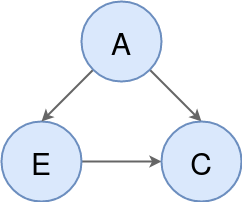
\includegraphics[scale=0.35]{Chapter2/Figs/example-dag.png}
    \caption{Ejemplo de un grafo causal $\mathcal{D}$ que representa el efecto del ejercicio $E$ sobre la salud $C$ y de la edad $A$ sobre ambos.}
    \label{fig:dag-causal}
\end{figure}
% \begin{itemize}
%     \item Definición de causalidad.
%     \item El por qué de los modelos causales, ventajas sobre enfoques asociativos
%     \item Escalera de la causalidad
%     \item Definición de causalidad según Pearl y  Spirtes
    
%     \item Conexión entre grafos y probabilidades
%     \item Modelos gráficos causales
%     \item Intervenciones y efectos 
%     \item Obtención de DAG
% \end{itemize}
% he termcausalityisdefined in terms of common language and then the mathematical machinery required to modelcausality is provided. In this way, causality becomes defined as whatis modeled by causalmodels, which are themselves defined as to model causality. This apparent circularity is deeplystudied by Woodward (2003). 


% We adopt themanipulationistintepretation of Causality as described in Woodward (2003).According to the definition from Spirtes et al. (2000), causality is defined as astochasticrelation betweenevents. The intuition is that some event (or events)causesanother event tooccurr according to some underlying mechanis


% Definition 2.1.Let (Ω,F,P) a finite probability space, and consider a binary relation→⊆F × Fwhich is:•Transitive: IfA→BandB→Cfor anyA, B, C∈ FthenA→C.•Irreflexive: For allA∈ Fit doesn’t hold thatA→A.•Antisymmetric: ForA, B∈ Fsuch thatA6=BifA→Bthen it doesn’t hold thatB→A.We will say thatAisa causeofB(or thatAcausesB,Ais the cause andBis the effect) ifA→B. It is important to note that an event may have more than one cause, and that notnecesarily each one of this causes is sufficient to produce the effe0ct

% The causal relations contained in→can be summarized in a graphG= (V, E) in the followingway: IfA→Bthen the graph must contain a nodeA∈VrepresentingA, a nodeB∈VrepresentingBand a directed edgee∈Econnecting the respective nodes in the direction ofthe causal relation

\subsection{Intervenciones y efectos causales}

% La probabilidad condicional $P(Y=y| X=x)$ da la probabilidad de que $Y$ tome el valor $y$, dado que se \textit{observó} que $X$  tomo el valor $x$. 
% Sin embargo, a menudo es de interés predecir el valor de $Y$ que resultará
% si se \textit{interviene} al fijar el valor de $X$ a un valor $x$ en particular. Esto último se denota como $P(Y=y| do(X=x))$ \cite{pearl_2009}.
¿Cuál es la diferencia entre observar e intervenir o
manipular? 
Cuando se interviene una variable en un modelo, se fija su valor y se elimina el efecto de sus padres, con esto se modifica el sistema y como resultado, normalmente, los valores de las otras variables cambian.
Por otra parte, cuando se condiciona sobre una variable, nada cambia, simplemente se limita el enfoque al subconjunto de casos en los que variable toma el valor de interés. 
% Por lo tanto, lo que cambia es la percepción del mundo, no el mundo mismo.

Para distinguir los casos donde una variable $X$ toma un valor $x$ naturalmente
y aquellos donde se fija $X = x$, este último se denota como $do(X=x)$.
Por lo tanto $P(Y=y|X=x)$ es la probabilidad de que $Y = y$ condicionado a 
observar $X=x$, mientras que $P(Y=y|do(X=x))$ es la  probabilidad de que $Y=y$
cuando se hace la intervención $X=x$.


En términos de distribuciones, $P(Y = y|X = x)$ refleja la distribución 
de la población de $Y$ entre individuos donde $X=x$.
Por otra parte, $P(Y = y|do(X = x))$ representa la distribución de
la población de $Y$ si todos en la población tuvieran el valor de $X$ fijado a
$x$ y eliminando el efecto de los padres de $X$ sobre ésta.
De manera similar, $P(Y = y|do(X = x), Z = z)$ sirve para denotar
la probabilidad condicional de $Y = y$, dado $Z = z$, 
en la distribución creada por la intervención $do(X = x)$.
% Cuando simplemente se observa el valor que una variable toma, se está aprendiendo acerca del valor de la 
% variable cuando ésta es causada de la manera normal, así como se está representada en el modelo causal.
% La información sobre el valor de la variable también provee
% datos sobre sus causas y sobre otros efectos de esas causas.

Cuando se hacen \textit{intervenciones},
se sobrescribe la estructura causal normal. Se obliga a una
variable a tomar el valor que no podría haber tomado 
si el sistema se quedara sin modificaciones.
Gráficamente, se puede representar el
efecto de esta intervención eliminando las aristas 
dirigidas a las variables que se desean intervenir. Tal
intervención a veces es descrita como ``romper'' esas aristas \cite{sep-causal-models}.

Dadas tres variables, $X$, $Y$ y $W$,
el efecto causal de $X$ sobre $Y$ se denota como $P(Y=y|do(X=x), W=w)$. Para 
cada realización $x$ de $X$, $P(Y=y| do(X=x), W=w)$ es la probabilidad de $Y=y$ 
inducida al eliminar del modelo todas las ecuaciones que corresponde a las
variables en $X$, sustituir $X=x$ en el resto de ecuaciones y observar los valores que toma otra variable, $W=w$, en el mismo ``mundo'' donde la intervención se lleva a cabo.
En general, si $X$ y $Y$ pueden tomar más de un valor, se desea poder
predecir el \textit{efecto causal general}.
La diferencia $\mathbb{E}(Y|do(x'))- \mathbb{E}(Y|do(x''))$ a veces
se toma como la definición de efecto causal general \cite{theoryofcausalities2006, pearl2016causal}
donde $x'$ y $x''$ son dos realizaciones diferentes de $X$.

Siguiendo el ejemplo de la Figura \ref{fig:dag-causal}, se puede intervenir
el modelo para calcular el efecto causal de las horas
de ejercicio sobre la salud del corazón. El efecto causal de $E=e$ puede 
verse como la distribución $P(C | do(E=e))$ sobre el grafo sin la arista
dirigida $A \rightarrow E$ (Figura \ref{fig:dag-intervention}) y sin alterar los otros parámetros ($P(A), P(C|E, A)$).

\begin{figure}
    \centering
    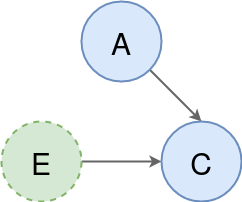
\includegraphics[scale=0.35]{Chapter2/Figs/example-dag-intervention.png}
    \caption{Ejemplo de un grafo causal sobre el cual se hace una intervención de
    la variable $E$. Se elimina la arista $A \rightarrow E$.}
    \label{fig:dag-intervention}
\end{figure}
% Supóngase que se tiene
% un modelo causal en el cual la distribución de 
% probabilidad $P$ satisface la condición de Markov en el 
% grafo causal $D$ sobre el conjunto de variables
% $\mathcal{V} = \{X_1, X_2,  \dots, X_n\}$.

% . The most useful version of MC for thinking about interventions is MCFactorization (see Section 3.3), which tells us:
% P(X1,X2,…,Xn)=∏iP(Xi∣PA(Xi))

% Now suppose that we intervene by setting the value of Xk
% to xk. The post-intervention probability P′

% is the result of altering the factorization as follows:
% P′(X1,X2,…,Xn)=P′(Xk)×∏i≠kP(Xi∣PA(Xi)),

% where P′(Xk=xk)=1
% . The conditional probabilities of the form P(Xi∣PA(Xi)) for i≠k remain unchanged by the intervention.


\section{Causalidad y aprendizaje por refuerzo}

De acuerdo con algunos trabajos, la relación entre el aprendizaje por refuerzo
y la causalidad es mucho más estrecha que con otras áreas del
aprendizaje automático, por lo que trabajos recientes
se han enfocado en conectar ideas de ambas
áreas \cite{Gershman2017, 6-DBLP:journals/midm/YuDLR19, lu2018deconfounding, dasgupta2019causal, schlkopf2019causality}.
 En este documento, más que intentar construir los fundamentos de una nueva 
teoría que combine ambas áreas, se apunta hacia una perspectiva
en la que elementos de una auxilien a la otra de tal forma que
los aproveche y mejore. En particular, en esta investigación
se sigue la dirección de utilizar información causal para ayudar al 
aprendizaje de un agente.

% Esto debido a que al ejecutar acciones sobre su ambiente, entonces
% estima distribuciones intervencionistas y por lo tanto el aprendizaje por refuerzo es un problema causal. Sin embargo, se ha demostrado que el aprendizaje
% por refuerzo no está formulado tal que se utilicen operaciones
% causales \cite{gonzalezsoto2019reinforcement}.
% En este documento, más que intentar construir los fundamentos de una nueva 
% teoría que combine ambas áreas, se apunta hacia una perspectiva
% en la que elementos de una auxilien a la otra de tal forma que
% los aproveche y mejore. En particular, en esta investigación
% se sigue la dirección de utilizar información causal para ayudar al 
% aprendizaje de un agente.

% Por esta razón, no se presentan conceptos teóricos que unan ambas áreas. 
% En capítulos posteriores se introducen algunas definiciones y notación
% que sirven para entender el método propuesto y que sirven para acotar el
% problema atacado.
% La mayoría de los algoritmos de aprendizaje por refuerzo son métodos genéricos que pueden ser aplicados a cualquier tarea modelada como un proceso de decisión de Markov.
En específico, esta investigación se restringe a hacer frente
a problemas que pueden ser planteados como un proceso de decisión de Markov condicionado a metas
\cite{nair2019causal}. Esto, debido a que de acuerdo  con la definición propuesta por \cite{nair2019causal} este 
tipo de tareas tiene una estructura causal subyacente que describe el comportamiento del ambiente.

    Un MDP condicionado a metas es
una tupla $<\mathcal{S}, \mathcal{A}, \mathcal{X},
\mathcal{D}, \mathcal{P}, \mathcal{G}, r, \gamma, \phi>$, donde 
\begin{itemize}
    \item $\mathcal{S}$ es el espacio de estados, 
    \item $\mathcal{A}$ es el espacio de acciones, 
    \item $\mathcal{X}$ es el conjunto de
    macro-variables de estado \cite{chalupka2014visual} (variables 
    que describen a los estados en un alto nivel), donde $|\mathcal{X}| = N$ y
    $N \ll |S|$, 
    \item $\mathcal{D}$ es un grafo causal
    que define relaciones entre
    los conjuntos $\mathcal{A}$ y $\mathcal{X}$, 
    \item $\mathcal{P}: \mathcal{S} \times \mathcal{A} \times \mathcal{S} \rightarrow [0, 1]
     $ es la función de probabilidad de transición de pasar de un estado a otro dada una acción. 
    \item $\mathcal{G}$ es el espacio de metas, donde cada uno de sus elementos es un vector $\mathbf{g} = [x_1, \dots, x_N]$ y $x_i \in \mathcal{X}$
    con $i \in \{1, \dots, N\}$,
    \item $r : \mathcal{S} \times \mathcal{A} \times \mathcal{G} \rightarrow \mathbb{R}$ es una función
de recompensa, donde $r(s, a, \mathbf{g})$ produce la recompensa inmediata condicionada a la meta $\mathbf{g} \in \mathcal{G}$,
\item $\gamma$ es el factor de descuento,
\item $\phi : \mathcal{S} \rightarrow \mathcal{X}$ es una función que relaciona el espacio de estados con el de macro-variables.
\end{itemize}

En un MDP condicionado a metas, el objetivo es aprender una 
política óptima condicionada a una meta $\pi^*_g: \mathcal{S} \times \mathcal{G} \rightarrow \mathcal{A}$ que maximice el retorno esperado $R = \sum_{k}^{\infty}\gamma^{k} r(s_k, a_k, g)$.

La definición y notación de MDP condicionado a metas
permiten entender el método propuesto y que sirven para acotar el problema atacado en los siguientes capítulos.